\documentclass[12pt]{article}

\usepackage{graphicx}
\usepackage{adjustbox}
\usepackage{enumitem} % to get rid-off extra spacing and more control

% Line spacing
\usepackage{setspace}
\setstretch{1.15}

% Times New Roman font
\usepackage[T1]{fontenc}
\usepackage[utf8]{inputenc}
\usepackage{mathptmx}

% Margins
\usepackage[top=0.8in, bottom=0.8in, left=0.8in, right=0.5in]{geometry}

% Shift Title up
\usepackage{titling}
\setlength{\droptitle}{-5em}   % This is your set screw

\title{``No, it just cannot be a Solid''} % Your article title
\author{Yogesh Kulkarni\\Dept. of Mech. Engineering, College of Engineering Pune, India} % Your name
\date{} % Add a date here if you would like one to appear underneath the title block

%----------------------------------------------------------------------------------------

\begin{document}

\maketitle
\vspace{-10mm}
%\begin{flushright}
%{\em Just as men breathe, as eagles sustain themselves in the air,\\
%Euler calculates without any apparent efforts.\\
%-  François  Arago (French Mathematician)}
%\end{flushright}

{\em - ``The shape I have has 20 vertices, 30 edges and 11 faces. Can you tell me if it is a closed Solid or an open Surface'?''} - an invisible voice asked.

%\bigskip

I said, {\em - ``What?? $\ldots$ ridiculous $\ldots$ how do I know? You haven't shown me the shape yet.''}

%\bigskip

But then, Mr. Euler, standing beside me, said, {\em - ``No, it just cannot be a Solid''}.

%\bigskip

While trying to suppress my amusement, I questioned {\em - ``How do you know for sure? Surely you are joking, Mr. Euler. Aren't you?''}.

%\bigskip

Mr. Euler quietly and convincingly said {\em - ``If you add just one more face, chances are that you CAN get a closed Solid''}.

%\bigskip

Regaining my balance, I shouted with astonishment {\em - ``Wow!! That is just amazing. Without looking at a shape, how in the world, you are able to tell me if it can be a closed Solid or not. This is no less than magic''}.

%\bigskip

By just knowing the number of vertices, edges and faces, one can predict whether it will be a closed Solid or not by Euler's formula $v - e + f = 2$. Ridiculously simple, isn't it? But then, this took more than 2000 years for mankind  to come  up with such a simple equation, which is now one of the most fundamental equations of Geometric Modeling.

\section*{Introduction}
\begin{tabular}{  p{0.5\linewidth}  p{0.35\linewidth} }
Greeks {\em discovered} solids around 4th century BC in the form of regular polyhedrons, such as tetrahedrons, cube, octahedron, \mbox{dodecahedron} and icosahedron, popularly known as {\em Platonic Solids} after Plato. Euclid gave comprehensive treatment to these solids in his famous book called {\em ``The Elements''}. But there was no generalization in terms of proving their ``Solid-ness'', which Euler did in the 18th century.
&
\centering  \resizebox{-0.65\linewidth}{!}{
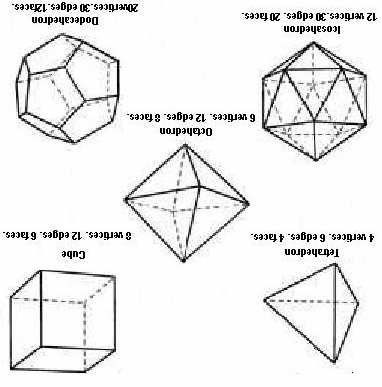
\includegraphics[width=\linewidth]{images/platonic.png}
}\\
\end{tabular}

Leonhard Euler can be easily regarded as the most significant mathematician of all times, due to his prolific work in areas as varied as calculus, analysis, number 
theory, topology, algebra, geometry, trigonometry, analytical mechanics, hydrodynamics, astronomy, light-sound-heat, cartography and graph theory.

\section*{Life and Works}

\begin{tabular}{  p{0.3\linewidth}  p{0.65\linewidth} }
\resizebox{-0.8\linewidth}{!}{
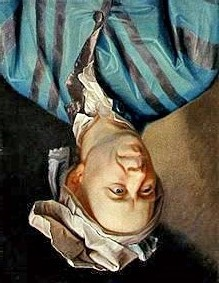
\includegraphics[width=\linewidth]{images/Euler}
}
&
Euler was born on 15th April 1707 in a Swiss town called Basel, where even the Bernoulli family lived. Johann Bernoulli got impressed with this mathematical prowess right from childhood and taught him throughout his later years. Forced by his father, Euler studied theology and got the masters degree at a tender age of 17 (equivalent to 11th standard for us). Later, he had to shift to Russia, first to do some odd jobs but later to become the chief mathematician at St. Petersburg Academy. During his stay in Russia, the government asked him to work on things like writing textbooks for schools, improving accuracy of weights, making maps, etc. but he did all this with great involvement and accuracy. 
\\
\end{tabular}

While working on maps, he stumbled upon the famous problem of ``7 bridges of Koenigsberg'', where one has to cross all the bridges only once and come back to the start point.

\begin{tabular}{  p{0.45\linewidth}  p{0.45\linewidth} }
%\resizebox{-0.9\linewidth}{!}{
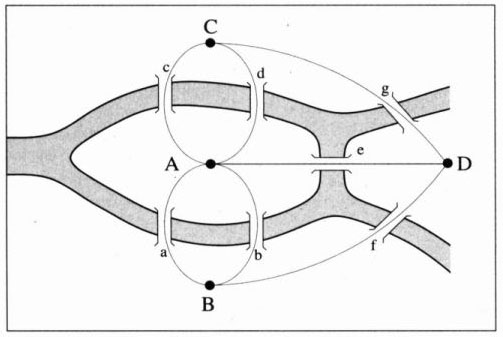
\includegraphics[width=0.8\linewidth]{images/bridges}
%}
&
%\resizebox{-0.9\linewidth}{!}{
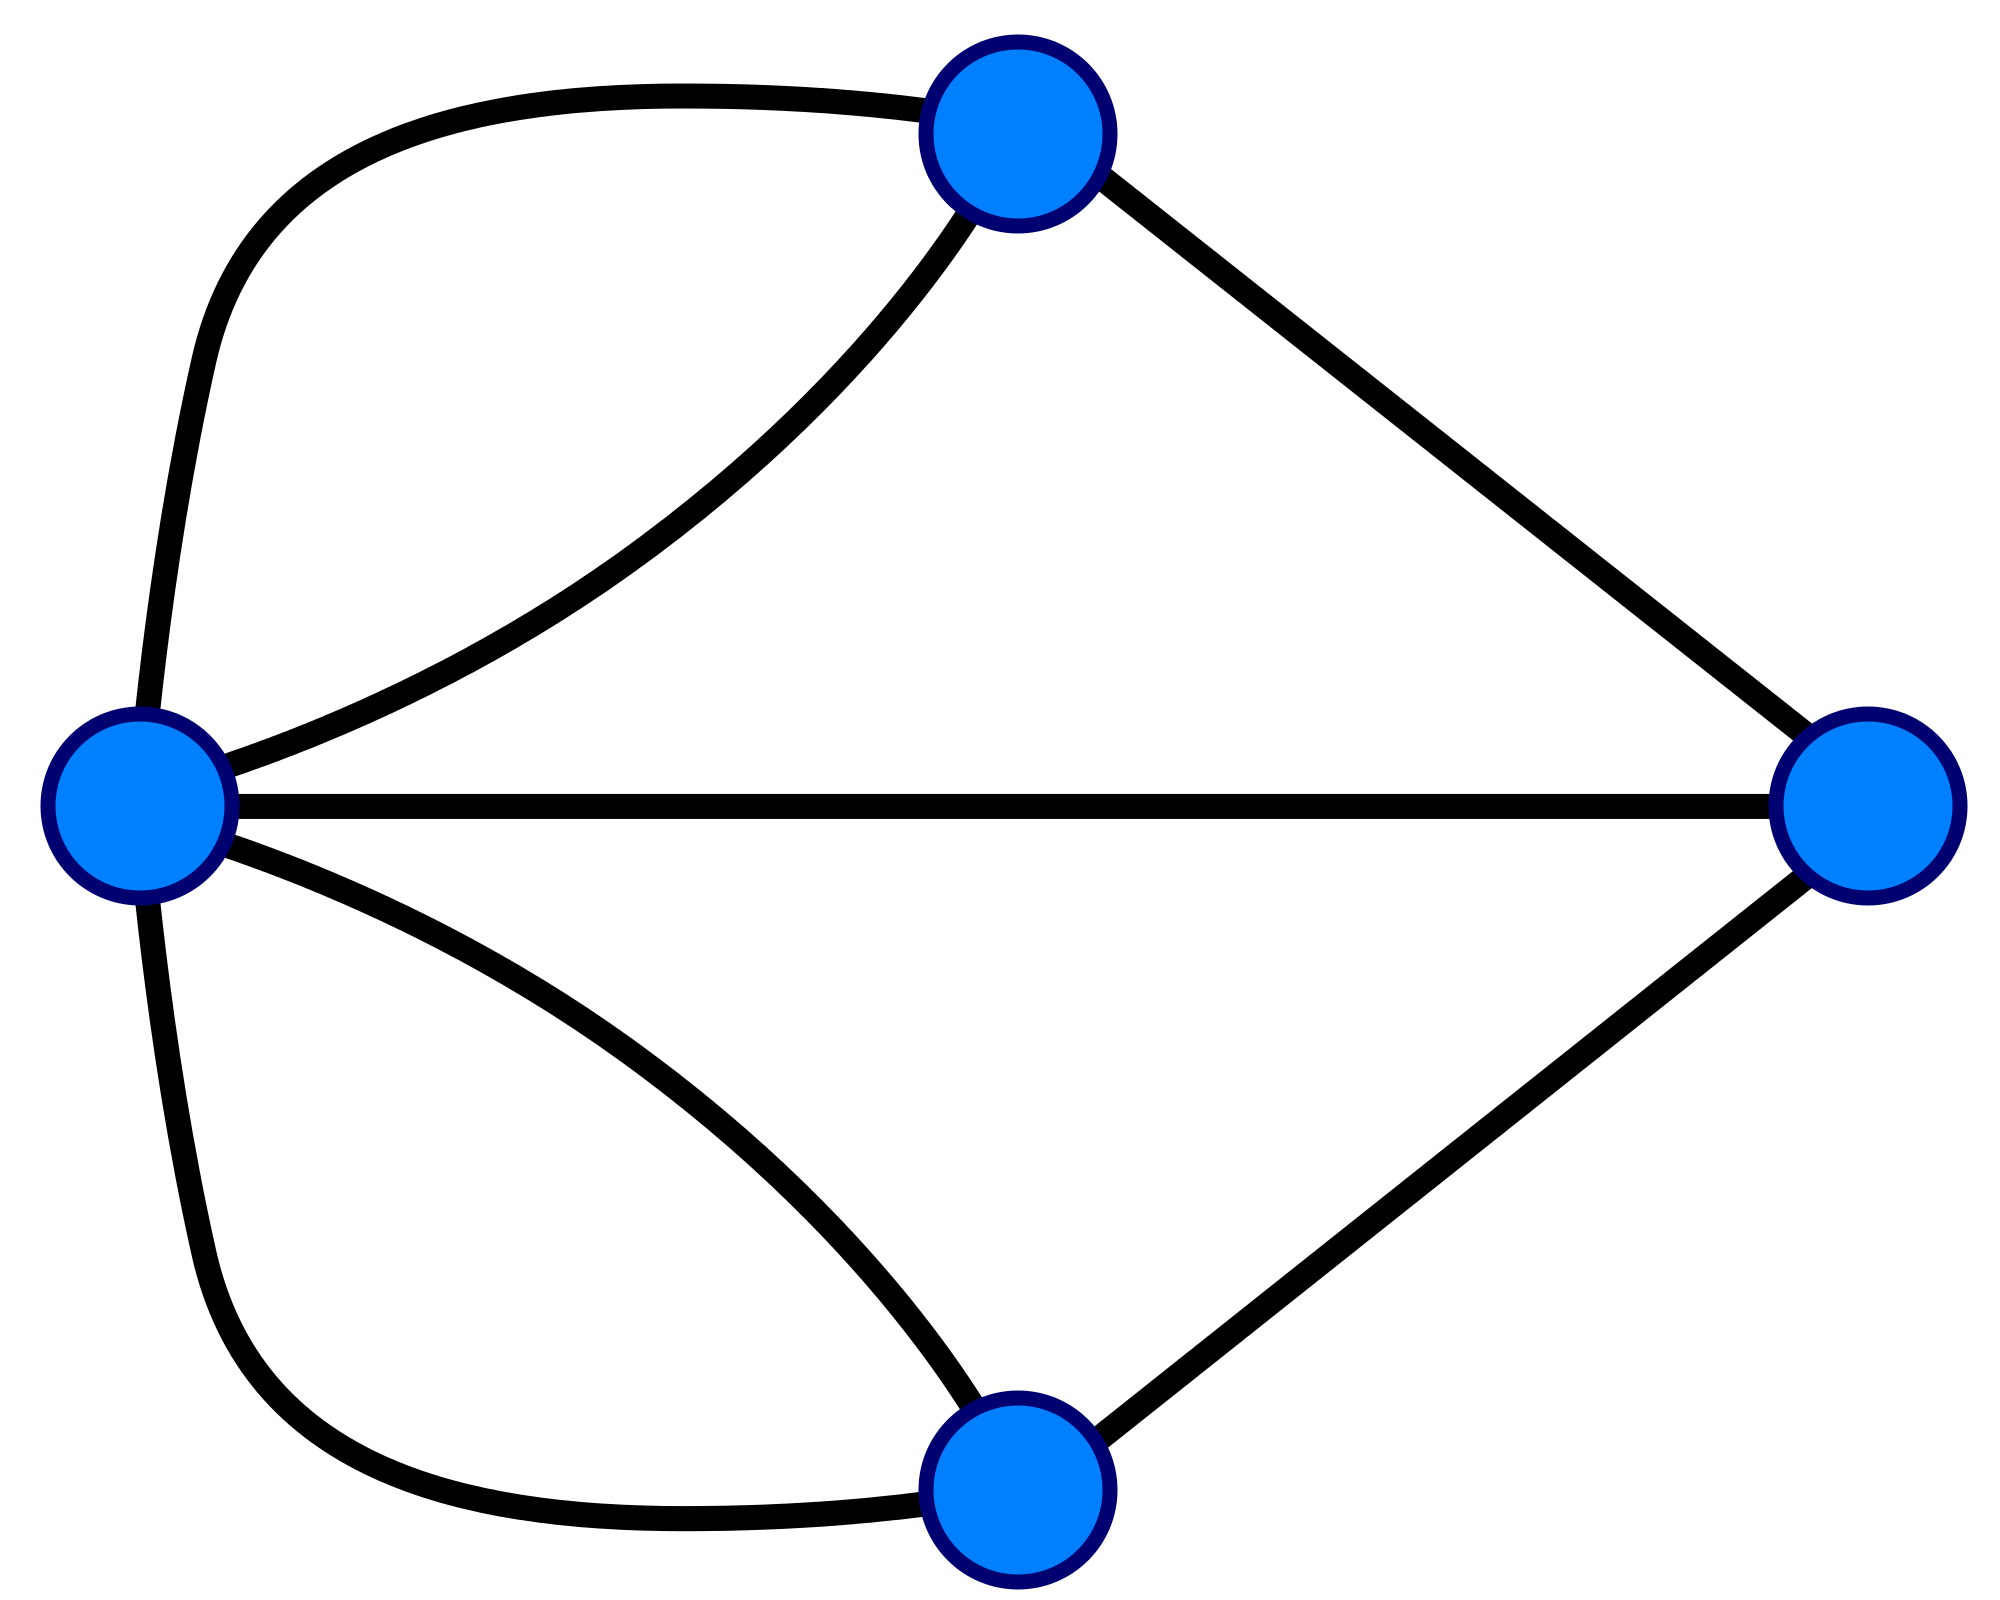
\includegraphics[width=0.6\linewidth]{images/graph}
%}
\\
\end{tabular}

Euler showed that it is not possible to do so as the network (graph) had $\ge 2$ odd vertices. He went ahead to show that if we relax the condition of  ``coming back to the original point'' (and retain ``crossing each bridge only once'') than it is possible if there are $2$ odd points. This path is called as ``Euler Path''. This theory got blossomed into the very popular ``graph theory'', thereby finding applications in Computer Science, Electric-Road networks, Operations Research, etc.

Euler worked extensively in the Number Theory. Fermat had proclaimed that $2^n + 1$ can be used to find prime numbers where $n$ has to be a power of 2. Euler proved him wrong by showing that for $n=32, 2^{32}+1 = 4294967297$ which is divisible by $641$.  Euler tried his hand at Fermat's last theorem ($a^n + b^n = c^n$ is true only for $n=1,2$ but not for further values of $n$) but did not succeed. Euler also tried proving Goldbach's conjecture (any even number can be written as a  sum of two prime numbers, for example, 12 = 5 + 7, 8 = 5 + 3) but could not do so.

One of the prominent discoveries by Euler are the properties of a constant called $e$, now called as ``Euler Constant''. We know this by a popular graph called ``exponential growth'' represented by $y = e^x$. He also devised formulas like $e^{i\pi} + 1 = 0$ and $e^{ix} = \cos x + i \sin x$.

Newton's and Leibniz's usage of functions was limited to equations. Euler proposed to use procedures or algorithms as functions. That's why he is also called as the first Algorist.

Euler brought Newton's laws of motion to the common man by his famous book called ``Mechanica''. He used calculus to calculate the capacity of beams, effect of air on trajectories, fluid flow, etc. He also worked with Daniel Bernoulli on thermal problems.

In the later part of his life, which he spent in Berlin, he  worked for Frederick the Great on problems like laying pipelines, ship navigation, pension tables, etc. Here, he wrote one of the classics called ``Calculus of Variations'', which fetched him membership of the London Royal Society and Paris Academy.

Towards the end, he went back to Russia where the queen gave him a palatial home to accommodate his large family!!

Till his last moment, he was mathematically active. At 77, on 18th September 1783, while drinking tea and solving problems, he died due to brain hemorrhage.


\section*{His devotion}
Euler breathed and lived mathematics, day and night. He wouldn't even spare a moment for relaxation. While working on a problem posed by the Paris Academy, he worked so relentlessly for 3 days (and nights) that he lost sight of one of his eyes. About half of Euler's mathematics was conceived, when he turned blind. His strong memory and sharp intellect made him continue his beloved work. One anecdote - one of his students was adding 17 numbers in a series, in which, Euler sensed some problem, and so he calculated that sum of large numbers in his mind itself!!

Euler was a wonderful teacher as well. He taught science and mathematics to a niece of the German King,  through letters, 234 of them!! This, then, got published as a book and made him world-famous. Euler wrote ``The Elements of Algebra'' to popularize the Number theory, Analysis, and of course, Algebra. Euler even wrote `` Mathematics in Music''. Mathematicians thought it was for musicians and vice versa, so probably, both did not read it. His volume of work is still not fully published. Swiss Association for Natural Sciences has started publishing his work from 1910 and it is still not over!!


\section*{Take-away}
Euler was a very simple man with no enemies. He did not get involved in debates or conflicts. He always helped others and never aimed for success. A real {\em nishkam karmayogi}.

Euler is an epitome of dedication to the subject. In-spite of turning blind and prevalent hostile surroundings, his loyalty or love for mathematics never faded. It is said, he worked so much that, whatever work on mathematics, mathematical  physics and engineering mechanics was discovered in the 18th century, Euler's was $\frac{1}{3}$ of it!!!

Euler's mathematics does not stop with him. More development is going on in all the fields that he started. Now let's go back to his Polyhedron formula and see if it works for a Solid having a hole!!



\section*{References}
\begin{enumerate}[noitemsep,nolistsep]
\item ``Roots of Geometry and Topology'' - Max Planck Institute Informatik
\item ``Ganiti'' - Achyut Godbole, Madhavi Thakurdesai
\end{enumerate}
\end{document}